\chapter{Conclusion}
\label{chap:conclusion}

This dissertation presents a motion planning approach suited for
multi-step manipulations tasks.
Key to the approach are the complementary ideas of \emph{lazy}
and \emph{utility-guided} search,
which we integrated into the LEMUR motion planning algorithm.
This concluding chapter begins by summarizing the dissertation
and the individual algorithmic contributions
in Section~\ref{sec:conclusion:summary}.
This is followed by a discussion in Section~\ref{sec:conclusion:future}
of a few promising avenues for future research
which build on our results.
Finally, we offer some concluding remarks
in Section~\ref{sec:conclusion:remarks}.

\section{Summary and Contributions}
\label{sec:conclusion:summary}

The central contribution of this dissertation is a collection of
algorithms which efficently implement an approach to motion planning
which explicitly addresses the inherent tradeoff between planning
and execution costs via a utility-guided search,
and then conducts its search lazily in order to minimize resources
while accomplishing the task.
We present an outline of the algorithms presented in this dissertation,
along with the interrelationships between them,
in Figure~\ref{fig:conclusion:outline}.

\begin{figure}
   \centering
   \includegraphics{build/outline}
   \caption{Outline of the algorithms developed in this dissertation.
      LEMUR is solves a continuous motion planning problem via
      discretization as a series of progressively densified roadmaps
      (Chapter~\ref{chap:roadmaps}).
      Since the shortest path problem over the resulting graph
      in characterized by edge costs which are expensive to evaluate,
      we exploit lazy search and edge selectors
      (Chapter~\ref{chap:lazysp}) to minimize planning effort.
      We also develop a novel incremental bidirectional search
      algorithm (Chapter~\ref{chap:ibid}) to accommodate the resulting
      dynamic pathfinding problem.
      LEMUR conducts its search guided by a utility function
      (Chapter~\ref{chap:utility}) which can employ distinct
      domain-specific planning and execution cost heuristics.
      In multi-step manipulation tasks,
      one such cost model is derived from the family motion planning
      problem (Chapter~\ref{chap:family}),
      which leads to planner invocations which minimize combined
      planning and execution cost.
      }
   \label{fig:conclusion:outline}
\end{figure}

Here I write about the conclusion!

We have proposed a motion planning approach for motion planning
using lazy search conducted over densified roadmaps
which maximizes utility using domain-informed
planning and execution cost heuristics.
This approach has shown promising results on manipulation tasks
when compared with state-of-the-art
search-based and sampling-based anytime planners.

We did these things.

\paragraph{Motion Planning via Roadmaps.}

Exploited roadmaps because of their good properties
in Chapter~\ref{chap:roadmaps}.
Can be cached.
Can be progressively densified.
We talk about ways to improve them later in the discussion.
Roadmaps are easy to parallelize.

Talk about distance functions.
Opportunity to optimize them as a function of the collision
probability in different parts of the space,
or in terms of the maximal Jacobian value over the arm
(bent elbow example).

Progressive densification is a proxy for handling the
spatial coherence in the scene.

\paragraph{How should we optimize?}

What should we do in the face of expensive state validity checking?

Once we commit to a discretization,
we take advantage of the planning cost structure
by conducting a lazy search.
We outline the LazySP algorithm.
This enables different edge selectors
which we discuss in Chapter~\ref{chap:lazysp}.

Conducting a lazy search produces an underlying dynamic shortest
path problem.
In particular, in some cases our estimate $w_{\ms{est}}$
may not be great.
This motivates us to look at approaches which are both
bidirectional and incremental.
This leads to the development of the IBiD algorithm.
We show that this has good performance,
both for road network routing and motion planning examples.

What is the effect of the tradeoff
between bidirectional and incremental search,
when a good heuristic is not available?

\paragraph{What should we optimize?}

Next,
we consider what we should be optimized in order to capture
the inherent tradeoff in manipulation tasks
between planning and execution cost.
We apply the concept of utility,
first described in BUGSY,
to the lazy search regime for the motion planning problem.

Utility allows domain-specific planning cost estimates
to be leveraged.

One example is a family of sets.
In Chapter~\ref{chap:family},
we talk about the family motion planning problem,
and give some examples where it is applicable.

\section{Future Directions}
\label{sec:conclusion:future}

\paragraph{Discussion.}
The remainder of this chapter discusses both the implications
and limitations of the presented approach,
as well as possible directions for future work.

In this chapter,
we discuss opportunities to extend our approach to acheive even
better performance,
examine options to better integrate motion planning into a
task planning system,
and expound on other promising future directions.

\subsection{Roadmaps}

Smarter sequences that are easy to densify.
Fractal patterns?
Not lattices.

\subsection{LazySP and Edge Selectors}

Faster ways to maintain the partition selector.
Locate pinch points (crux evaluation).

Dynamically balance between sides?
Where is the maze?

\subsection{Incremental Bidirectional Search}

When used by LazySP,
if we do forward,
can we dynamically adjust the distance balance criterion
so that the location of the dynamic interface
matches the radius of the update?

How to do balanced cardinality with incremental search?

\subsection{Approaches for Roadmap Densification}

One of the fundamental questions in any motion planning approach
is how should the continuous problem be approximated in order
to search for a solution.
Usually,
this is accomplished through discretization.

We first consider some possible extensions to the core
LEMUR planner from Chapter~\ref{chap:utility}.
First, what kind of roadmap should be used
(Section~\ref{sec:discussion:disc})?
This is a fundamental question because it specifies how the
continuous problem is discretized.

\subsection{Adaptive Roadmap Densification via an Infinite Roadmap Stack}
\label{sec:discussion:disc}
The LEMUR planner effectively conducts its search over a sequence of
progressively densified roadmaps
(Figure~\ref{fig:discussion:roadmap-stack}).
The results presented in this thesis have used Halton sequences
as discussed in Chapter~\ref{chap:roadmaps}
for their prefereable dispersion properties,
and form a roadmap graph using an $r$-disk connection rule.
As discussed in \citep{janson2015deterministicsampling},
the shorest path on such a sequence of roadmaps
posesses asymptotic optimality if the connection radius is adjusted
appropriately.

\begin{figure}
   \centering
   \includegraphics{build/roadmap-stack}
   \caption{A stack of progressively densified roadmaps
      over a given free configuration space $\mathcal{C}$.}
   \label{fig:discussion:roadmap-stack}
\end{figure}

\paragraph{Hard batching.}
Like many existing roadmap-based algorithms
\citep{starek2015bfmtstar, gammell2015bitstar},
LEMUR implements a hard batching approach to densification --
a search is conducted fully over each batch of the roadmap
in $\mathcal{C}$
until a solution is found.
While the specification of LEMUR allows for this roadmap to be
implicitly constructed,
the current implementation constructs the entire batch before
proceeding with its search.
Once the search over that roadmap completes without a feasible path found,
the next batch of vertices and edges are added to the graph,
and the newly densified roadmap is searched.

Because the sequence of roadmaps that is searched is insensitive to
the distribution of obstacles,
the current implementation of LEMUR is able to pre-compute a sequence
of roadmaps up to a certain level of discretization,
and then load that roadmap structure into memory directly
instead of building it from scratch for each planning query.

There are two shortcomings that arise from this hard batching approach:

\begin{itemize}
\item \emph{Uniform Densification:}
   The fact that this roadmap is loaded uniformly across the space
   is certainly a limitation that will become restrictive
   in spaces of larger dimension.
\item \emph{Densification vs. Resolution Completeness:}
   The current LEMUR algorithm only moves to a denser roadmap
   once no finite paths are shown to be available on the present
   roadmap.
   This may not be desirable in large spaces --
   it may make sense to move to a denser roadmap in the vicinity of
   a short path before exploring all corners of the space.
\end{itemize}

There are a number of promising avenues for a solution
to the problems that arise from uniform densification..
Informed anytime algorithms
\citep{gammell2014informedrrtstar, gammell2015bitstar}
restrict densification once an initial path is found to a subset of
the full space that may contain better solutions.
This approach is not directly applicable
because LEMUR is not an anytime algorithm.

\paragraph{Adaptive Roadmap Densification.}
An alternative strategy is to adopt an adaptive densification approach
under which the search is conducted upon an infinite stack of
progressively densified roadmaps.

Consider the roadmap stack depicted
in Figure~\ref{fig:discussion:roadmap-stack-onramps}.
Here, as before,
each underlying roadmap is a superset of the one above it.
But now,
instead of progressively considering each layer individually
(using batching),
consider conductiong a single search over the entire stack.
Note that the stack includes additional edges
(shown dotted in the figure)
connecting corresponding vertices in two adjacent layers;
using a road network analogy,
we call these edges ``offramp'' edges.
A proposed edge weighting scheme involves two components:
(a) an artificial inflation of edge weights by some factor
on each layer according to a schedule
(with edges on lower layers inflated more),
and (b) an artificial constant weight assigned to each offramp edge
between layers.

%Related to the idea of adaptive dimensionality
%\citep{gochevetal2011adaptivedim}
%(large portions of solutions can be low-dimensional).

\begin{marginfigure}
   \centering
   \includegraphics{build/roadmap-stack-onramps}
   \caption{A roadmap stack with ``offramp'' edges.}
   \label{fig:discussion:roadmap-stack-onramps}
\end{marginfigure}

Consider a search over this infinite stack $G$
between two start and destination
configurations corresponding to distinguished vertices on $G$,
and consider an optimal solution path with strong $\delta$-clearance.
If the roadmap layers satsify the appropriate conditions
(e.g. connection radius
\citep{karaman2011samplingoptimal, janson2015deterministicsampling}),
and all roadmap edges have non-negative weight,
and all ``offramp'' edges have some constant positive weight $\alpha$,
then we conjecture that there exists a shortest path $p$ through $G$
of finite length (which traverses a finite number of layers of $G$).
Furthermore,
we conjecture that the length of $p$ approaches the length of an
optimal path as $\alpha \rightarrow 0$.

We find this representation of the continuous problem compelling
because it natually integrates the densification problem with
the search problem.
One can imagine a unidirectional or bidirectional search
effectively trading off between
exploring more widely on a particular layer
and descendng to a denser layer in order to traverse a narrow passage.
Descending to a denser layer occurs natually during the search,
and denser regions can be sampled on demand only in areas of the space
adjacent to obstacles blocking the path.
Furthermore,
the computational cost of such densification can be captured as
an additional planning cost component in the LEMUR algorithm,
so it will commit to a denser layer only when the predicted path
savings outweigh the requisite planning cost.

\subsection{Better Planning Cost Estimates}

The planning cost model we used for our experiments in this thesis
was very simple:
each collision check entails a constant amount of computational cost.
There are a number of ways that our model can be improved:
\begin{itemize}
\item The planning cost incurred by performing a collision check
   can be estimated dynamically,
   either across a planning episode,
   or as a function of the check's location in the C-space.
\item We can include planning cost models for additional aspects of
   the planner which can be costly.
   Two immediate candidates are
   (a) the cost of conducting an additional inner search
   over the lazy graph,
   and (b) the cost of progressing to a denser roadmap graph.
   Accommodating these estimates may lead to a more natural
   termination condition as well.
\end{itemize}

\subsection{Exploring the Interaction between Lazy and Dynamic Search}

Lazy search induces a dynamic shortest path problem,
as edge weights are updated and intermediate candidate paths are
required.
When LEMUR addresses a problem with $\lambda_p > 0$,
so that planning cost is to be considered in its utility objective,
it generally selects candidates that are no longer the fastest
to execute (e.g. the shortest) in the hopes of reducing planning time.

Paradoxically,
as the $\lambda_p$ parameter is increased,
the underlying dynamic search problem becomes more difficult,
because its heuristic is no longer as strong.
(A consistent heuristic typically only exists for the component of
the edge weight function derived from the execution cost component.)
It may would be beneficial to investigate schemes whereby
the requirement for optimal shortest paths from the inner
dynamic search is relaxed.
One suitable algorithm for this problem is Truncated
Incremental Search \citep{aine2016truncatedincremental}.

\subsection{Maximizing Utility in Expectation}

The LEMUR algorithm exploints an optimistic assumption when considering
candidate paths for prospective evaluation:
it assumes all unevaluated edges are collision-free.
While this assumption allows the inner loop to process candidates
quickly,
it requires the hard batching approach to strike an artificial
balance between local and global exploration.
It is worth investigating whether abandoning the optimistic
assumption is worthwhile --
a replacement would reason explicitly about the collision probability
across the configuation space.

We recently proposed a first step in this direction
via the Pareto Optimal Motion Planner \citep{choudhury2016pomp}.
In this work,
we maintain a probabilistic model of the probability of collision
across the configuration space,
which we update incrementally as collision checks are performed
agains the environment.
The planner then uses this model in order to select candidate paths
for partial evaluation that minimize some combination of the path's
execution cost and its probability of collision.



%\cdnote{Talk about Shushman's POMP stuff.}
%
%The purpose of the incremental graph densification strategy
%achieved by hard batching (Chapter~\ref{chap:utility})
%is to account for spatial correlation
%in $\mathcal{C}_{\mbox{\scriptsize free}}$.
%We would like to motivate this more formally.
%
%We propose to extend the E$^8$-PRM planner
%to minimize ensemble effort \emph{in expection}
%using a probabalistic model of $\mathcal{C}_{\mbox{\scriptsize free}}$.
%Even if this is too expensive,
%we can motivate the incremental densification idea,
%with a graduated cost model
%to approximate a probabalistic model
%of the $\mathcal{C}$-space.
%
%How should discrete graphs be constructed in continuous
%   $\mathcal{C}$-spaces with spatially correlated execution costs?
%
%Chapter~\ref{chap:graphs-in-continuous}
%discusses how to embed roadmaps in $\mathcal{C}$
%so that they can be searched by E$^8$.
%
%The problem with na\"{\i}vly running E$^8$ on a
%dense roadmap in $\mathcal{C}$
%is that it tends to bunch up in local minima.
%This is because reducing the continuous planning problem
%to a graph search ignores the spatial correlation
%inherent in $\mathcal{C}_{\mbox{\scriptsize free}}$.
%
%One way to capture this is to maintain a probabalistic model
%of $\mathcal{C}_{\mbox{\scriptsize free}}$,
%and then optimize in expectation.
%In particular,
%instead of greedily choosing the best path based on
%optimistic estimates of one-time planning and execution cost:
%\begin{equation}
%   f(\pi) = \lambda \hat{f}_p(\pi) + (1-\lambda) \hat{f}_x(\pi),
%\end{equation}
%we instead reason over the total \emph{expected} remaining cost:
%\begin{align}
%   f(\pi)
%      &= E \left[ \lambda f_p(\pi) + (1-\lambda) f_x(\pi) \right] \\
%   &= P_{\mbox{\scriptsize free}}(\pi)
%      \left[ \lambda \hat{f}_p(\pi) + (1-\lambda) \hat{f}_x(\pi) \right]
%      + (1-P_{\mbox{\scriptsize free}}(\pi))
%      \left[ \lambda F_p + (1-\lambda) F_x \right]
%\end{align}
%
%Consider the the problem from Figure~\ref{fig:example-in-expectation}.
%There are an infinite number of paths to the goal,
%each consisting of walking along the sidewalk,
%followed by crossing the street perpendicuarly at a particular
%position $x$.
%The sidewalk is known to be collision-free,
%whereas each position on the street must be tested for collision
%with obstacles with planning validation cost $\hat{f}_p(\pi)$
%independent of $x$.
%Execution cost $f_x(\pi)$ is given by $|x|+c$.
%
%Suppose we first test walking straight across the street $\pi_0$
%(knowing nothing, this is clearly the optimistically cheapest path)
%and this is deemed in collision.
%Which path should we consider next (e.g $\pi_a$ or $\pi_b$)?
%
%What is our model for $P_{\mbox{\scriptsize free}}(\pi)$?
%Relate to GPs for classification\cite{rasmussen2006gpml}.
%
%We are operating under assumptions:
%\begin{itemize}
%\item Single-shot greedy (won't choose \emph{sets} of paths
%   which minimize remaining effort)
%\item Operates over \emph{paths} instead of configurations
%   or edges (won't probe points, no explicit exploration)
%\end{itemize}
%
%\begin{figure}
%   \begin{center}
%   \includegraphics{build/example-in-expectation}
%   \end{center}
%   \caption{Simple example problem to illustrate optimizing
%      remaining ensemble cost in expectation.}
%   \label{fig:example-in-expectation}
%\end{figure}

\subsection{Integration with Collision Checking}

Most sampling-based planners consider the collision checker
to be a block box;
given a configuration $q_{\ms{test}}$,
this procedure considers the environment
and the robot's kinematics,
and returns a boolean answer -- True or False.
Depending on the fidelity of the geoemtric model of the robot
and environment,
each check can entail tens, hundreds, or even thousands
of microseconds;
precious planning time which can detract from the robot's overall
task performance.

One avenue for minimizing the computation effort spent performing
collision checks is integrate directly with the broad-phase
algorithm which effectively identifies configurations for which
many (or all) geometric pairs are sufficiently far from collision
that the more expensive narrow-phase checks need not be applied.

\begin{figure}
   \centering

   % left side
   \subfloat[Paths with lambda=0][%
      \centering
      Paths with $\lambda = 0$\par
      Average length: 733.0\par
      Average check cost: 7219.5
   ]{
      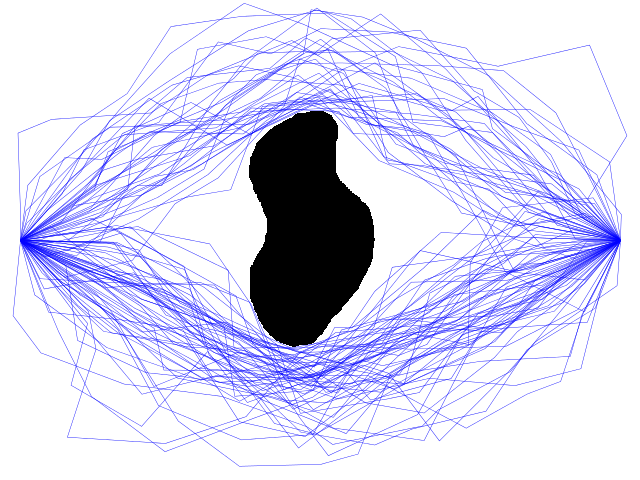
\includegraphics[width=0.45\textwidth]
      {figs/bean-allpaths-lambda0.png}
   }
   % right side
   \subfloat[Paths with lambda=1][%
      \centering
      Paths with $\lambda = 1$\par
      Average length: 836.5\par
      Average check cost: 4692.6
   ]{
      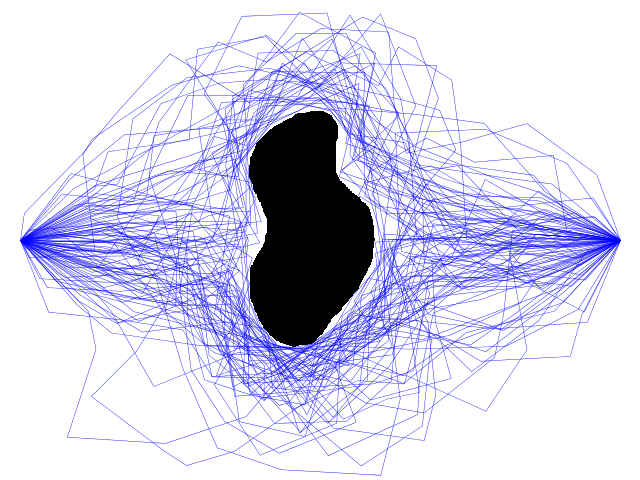
\includegraphics[width=0.45\textwidth]
      {figs/bean-allpaths-lambda1.png}
   }
   \\
   \subfloat[Paths with lambda=0][%
      \centering
      Paths with $\lambda = 0$\par
      Average length: 733.0\par
      Average check cost: 2685.7
   ]{
      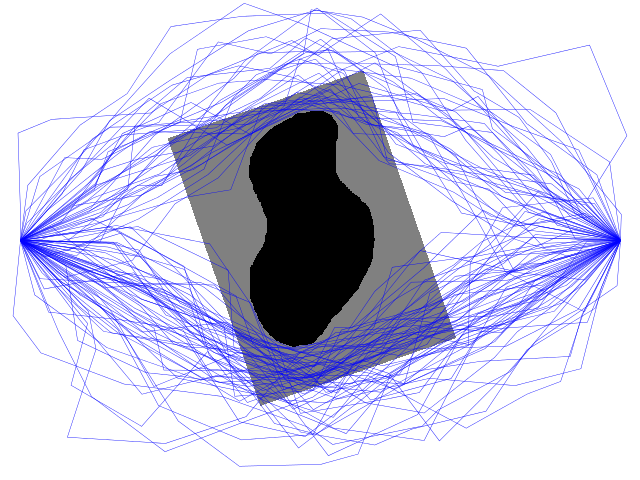
\includegraphics[width=0.45\textwidth]
      {figs/bean-allpaths-padded-lambda0.png}
   }
   % right side
   \subfloat[Paths with lambda=1][%
      \centering
      Paths with $\lambda = 1$\par
      Average length: 907.1\par
      Average check cost: 1064.5
   ]{
      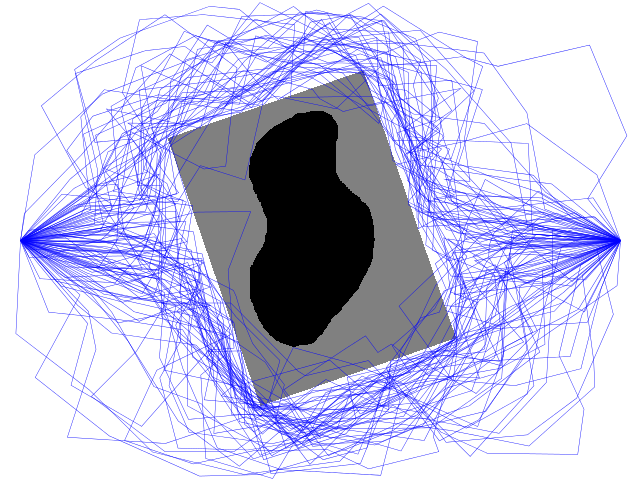
\includegraphics[width=0.45\textwidth]
      {figs/bean-allpaths-padded-lambda1.png}
   }

   \caption{A simple 2D example of the Multi-Set PRM using
     a broad-phase check.
     Checking for collision with the grey box is 10x less expensive
     than with the actual black obstacle.}
     %\cdnote{I need to talk about this in the text.}}
   \label{fig:broad-phase-2d}
\end{figure}

\begin{figure*}
   \centering
   
   \subfloat[
      A motion planner testing simply for membership in
      $\mathcal{C}_{\mbox{\scriptsize free}}$
      treats a collision validity checker as a
      ``black box.''
      Internally,
      modern checkers first employ an inexpensive broad-phase check
      using a low-dimensional conservative representation
      to quickly identify non-colliding bodies before
      resorting to an expensive narrow-phase check.
   ]{%
      \includegraphics{build/broadphase-single}%
   }%
   \quad%
   \subfloat[
      A family motion planner can explicitly reason about the
      conservative nature of the broad-phase check.
      This allows it to defer some narrow phase checks
      (often indefinitely)
      and instead prefer paths that require fewer expensive checks.
   ]{%
      \includegraphics{build/broadphase-multi}%
   }
   
   \caption[][0.0in]{Collision validity checking is a commonly used
     indicator function.
     The family motion planning formulation allows an intelligent
     planner to reach inside the checker's ``black box''
     and reduce the number of costly narrow-phase checks.
     Resulting paths tend to be cheaper to compute and
     stay further from obstacles.}
   \label{fig:broad-phase}
\end{figure*}

Consider the illustrative motion planning example shown
in Figure~\ref{fig:broad-phase-2d},
and the corresponding two-phase system described
in Figure~\ref{fig:broad-phase}.

\cdnote{
More caching!
Hypothesized volumes / Cell decompositions.
Bored robots.
Similarity to Leven/Hutchenson.
}

\subsection{Tighter Motion Planner Integration in a Planning System}

A motion planner is one component in a larger planning system for
an articulated robot performing real-world tasks.
There are opportunities for improved system performance by
integrating the planner more tightly with other system components.

\subsection{Integration with stuff above}

ISER task planning.
Cite ISER paper.

Task and motion planning.

I did some work on CMR stuff for multi-step problems,
for instance.
Cite this.

\paragraph{Task and Motion Planning.}
Other recent work has married symbolic reasoning with geometric planning
for tasks with multiple subtasks
as multi-modal planning \citep{hauser2010multi},
temporal logic \citep{bhatia2010temporalgoals},
or hierarchical or bridged representations and interfaces
\citep{cambon2009hybrid}, \citep{gravot2005asymov},
\citep{srivastava2014taskmotion}.

Treat an entire multi-step plan using LazySP (each edge is expensive after all!)

\paragraph{Other Applications of LazySP.}
\cdnote{Talk about satellite application from that guy.}

\section{Concluding Remarks}
\label{sec:conclusion:remarks}

Here are some concluding remarks.
